\documentclass{beamer}
\usepackage[utf8]{inputenc}
\usepackage{graphicx, epsfig}
\usepackage{amsmath,mathrsfs,amsfonts,amssymb}
\usepackage{floatflt}
\usepackage{epic,ecltree}
\usepackage{mathtext}
\usepackage{fancybox}
\usepackage{fancyhdr}
\usepackage{multirow}
\usepackage{enumerate}
\usepackage{epstopdf}
\usepackage{multicol}
\usepackage{algorithm}
\usepackage[noend]{algorithmic}
\usepackage{tikz}
\usepackage{blindtext}
\usetheme{default}%{Singapore}%{Warsaw}%{Warsaw}%{Darmstadt}
\usecolortheme{default}

\setbeamerfont{title}{size=\Huge}
\setbeamertemplate{footline}[page number]{}

\setbeamertemplate{section in toc}[sections numbered]


\makeatletter
\newcommand\HUGE{\@setfontsize\Huge{35}{40}}
\makeatother    

\setbeamerfont{title}{size=\HUGE}
\beamertemplatenavigationsymbolsempty

% latin bold lower
\newcommand{\ba}{\mathbf{a}} 
\newcommand{\bc}{\mathbf{c}} 
\newcommand{\be}{\mathbf{e}} 
\newcommand{\bh}{\mathbf{h}} 
\newcommand{\bp}{\mathbf{p}} 
\newcommand{\bt}{\mathbf{t}} 
\newcommand{\bs}{\mathbf{s}} 
\newcommand{\bu}{\mathbf{u}} 
\newcommand{\bv}{\mathbf{v}} 
\newcommand{\bw}{\mathbf{w}} 
\newcommand{\bx}{\mathbf{x}} 
\newcommand{\by}{\mathbf{y}} 
\newcommand{\bz}{\mathbf{z}} 

% latin bold upper
\newcommand{\bA}{\mathbf{A}} 
\newcommand{\bB}{\mathbf{B}} 
\newcommand{\bC}{\mathbf{C}} 
\newcommand{\bI}{\mathbf{I}} 
\newcommand{\bJ}{\mathbf{J}} 
\newcommand{\bL}{\mathbf{L}} 
\newcommand{\bM}{\mathbf{M}} 
\newcommand{\bP}{\mathbf{P}}
\newcommand{\bQ}{\mathbf{Q}} 
\newcommand{\bR}{\mathbf{R}} 
\newcommand{\bT}{\mathbf{T}} 
\newcommand{\bU}{\mathbf{U}} 
\newcommand{\bV}{\mathbf{V}} 
\newcommand{\bW}{\mathbf{W}} 
\newcommand{\bX}{\mathbf{X}} 
\newcommand{\bY}{\mathbf{Y}} 
\newcommand{\bZ}{\mathbf{Z}} 

% latin cal upper
\newcommand{\cF}{\mathcal{F}} 
\newcommand{\cG}{\mathcal{G}} 
\newcommand{\cI}{\mathcal{I}} 
\newcommand{\cL}{\mathcal{L}} 
\newcommand{\cM}{\mathcal{M}} 
\newcommand{\cN}{\mathcal{N}} 
\newcommand{\cP}{\mathcal{P}} 
\newcommand{\cS}{\mathcal{S}} 
\newcommand{\cT}{\mathcal{T}} 
\newcommand{\cW}{\mathcal{W}} 
\newcommand{\cX}{\mathcal{X}} 
\newcommand{\cZ}{\mathcal{Z}} 

% latin bb upper
\newcommand{\bbE}{\mathbb{E}} 
\newcommand{\bbI}{\mathbb{I}} 
\newcommand{\bbP}{\mathbb{P}} 
\newcommand{\bbR}{\mathbb{R}} 

% greek bold lower
\newcommand{\bepsilon}{\boldsymbol{\epsilon}} 
\newcommand{\btheta}{\boldsymbol{\theta}} 
\newcommand{\blambda}{\boldsymbol{\lambda}} 
\newcommand{\bpi}{\boldsymbol{\pi}} 
\newcommand{\bmu}{\boldsymbol{\mu}} 
\newcommand{\bsigma}{\boldsymbol{\sigma}} 
\newcommand{\bphi}{\boldsymbol{\phi}} 

% greek bold upper
\newcommand{\bSigma}{\boldsymbol{\Sigma}} 

\DeclareMathOperator*{\argmin}{arg\,min}
\DeclareMathOperator*{\argmax}{arg\,max}

\newcommand{\createdgmtitle}[1]{\title[\hbox to 56mm{Deep Generative Models  \hfill\insertframenumber\,/\,\inserttotalframenumber}]
	{\vspace{1cm} \\ \textbf{Deep Generative Models} \\ {\Huge Lecture #1}}
	\author{Roman Isachenko}
		\institute{
\includegraphics[width=0.7cm]{../utils/aimasterslogo} \LARGE{AI Masters}}
	\date{2024, Spring}
}

\usepackage{tikz}
\usetikzlibrary{arrows,shapes,positioning,shadows,trees}

\newcommand\myfootnote[1]{%
  \tikz[remember picture,overlay]
  \draw (current page.south west) +(1in + \oddsidemargin,0.5em)
  node[anchor=south west,inner sep=0pt]{\parbox{\textwidth}{%
      \rlap{\rule{10em}{0.4pt}}\raggedright\scriptsize \textit{#1}}};}

\newcommand\myfootnotewithlink[2]{%
  \tikz[remember picture,overlay]
  \draw (current page.south west) +(1in + \oddsidemargin,0.5em)
  node[anchor=south west,inner sep=0pt]{\parbox{\textwidth}{%
      \rlap{\rule{10em}{0.4pt}}\raggedright\scriptsize\href{#1}{\textit{#2}}}};}
      
\AtBeginSection[]
      {
      	\begin{frame}{Outline}
      		\tableofcontents[currentsection]
      	\end{frame}
      }
      \AtBeginSubsection[]{
      	\begin{frame}{Outline}
      		\tableofcontents[currentsection,currentsubsection]
      	\end{frame}
}
\createdgmtitle{14}

\usepackage{tikz}

\usetikzlibrary{arrows,shapes,positioning,shadows,trees}
%--------------------------------------------------------------------------------
\begin{document}
%--------------------------------------------------------------------------------
\begin{frame}[noframenumbering,plain]
%\thispagestyle{empty}
\titlepage
\end{frame}
%=======
\begin{frame}{Recap of previous lecture}
	\vspace{-0.2cm}
	\begin{block}{SDE basics}
		Let define stochastic process $\bx(t)$ with initial condition $\bx(0) \sim p_0(\bx)$:
		\[
			d\bx = \mathbf{f}(\bx, t) dt + g(t) d \bw, 
		\]
		where $\bw(t)$ is the standard Wiener process (Brownian motion)
		\vspace{-0.2cm}
		\[		
			\bw(t) - \bw(s) \sim \cN(0, (t - s) \bI), \quad d \bw = \bepsilon \cdot \sqrt{dt}, \, \text{where } \bepsilon \sim \cN(0, \bI).
		\]
	\end{block}
	\vspace{-0.5cm}
	\begin{block}{Langevin dynamics}
		Let $\bx_0$ be a random vector. Then under mild regularity conditions for small enough $\eta$ samples from the following dynamics
		\vspace{-0.2cm}
		\[
			\bx_{t + 1} = \bx_t + \eta \frac{1}{2} \nabla_{\bx_t} \log p(\bx_t | \btheta) + \sqrt{\eta} \cdot \bepsilon, \quad \bepsilon \sim \cN(0, \bI).
		\]
		will comes from $p(\bx | \btheta)$.
	\end{block}
	The density $p(\bx | \btheta)$ is a \textbf{stationary} distribution for the Langevin SDE.
	\myfootnotewithlink{https://www.stats.ox.ac.uk/~teh/research/compstats/WelTeh2011a.pdf}{Welling M. Bayesian Learning via Stochastic Gradient Langevin Dynamics, 2011}
\end{frame}
%=======
\begin{frame}{Outline}
	\tableofcontents
\end{frame}
%=======
\section{Probability flow ODE}
%=======
\begin{frame}{Probability flow ODE}
	\begin{block}{Stochastic differential equation}
		\[
			d\bx = \mathbf{f}(\bx, t) dt + g(t) d \bw
		\] 	
	\end{block}
	\begin{block}{Theorem (Kolmogorov-Fokker-Planck)}
 		\vspace{-0.2cm}
 		\[
 			\frac{\partial p(\bx, t)}{\partial t} = \text{tr}\left(- \frac{\partial}{\partial \bx} \bigl[ \mathbf{f}(\bx, t) p(\bx, t)\bigr] + \frac{1}{2} g^2(t) \frac{\partial^2 p(\bx, t)}{\partial \bx^2} \right)
 		\]
 	\end{block}
		\[
			d\bx = \left[\mathbf{f}(\bx, t) -\frac{1}{2} g^2(t) \frac{\partial}{\partial \bx} \log p(\bx, t) \right] dt = \tilde{\mathbf{f}}(\bx, t) dt
		\] 	
	\myfootnotewithlink{https://arxiv.org/abs/2011.13456}{Song Y., et al. Score-Based Generative Modeling through Stochastic Differential Equations, 2020}
\end{frame}
%=======
\begin{frame}{Probability flow ODE}
	\begin{block}{Kolmogorov-Fokker-Planck equation}
 		\vspace{-0.2cm}
 		\begin{multline*}
 			\frac{\partial p(\bx, t)}{\partial t} = \text{tr}\left(- \frac{\partial}{\partial \bx} \bigl[ \mathbf{f}(\bx, t) p(\bx, t)\bigr] + \frac{1}{2} g^2(t) \frac{\partial^2 p(\bx, t)}{\partial \bx^2} \right) = \\
 			=  \text{tr}\left(- \frac{\partial}{\partial \bx} \left[ \mathbf{f}(\bx, t) p(\bx, t) + \frac{1}{2} g^2(t) {\color{violet}\frac{\partial p(\bx, t)}{\partial \bx}} \right]  \right) = \\
 			 =  \text{tr}\left(- \frac{\partial}{\partial \bx} \left[ \mathbf{f}(\bx, t) p(\bx, t) + \frac{1}{2} g^2(t) {\color{violet}p(\bx, t) \frac{\partial \log p(\bx, t)}{\partial \bx}} \right]  \right)= \\
 			  =  \text{tr}\left(- \frac{\partial}{\partial \bx} \left[ \left( \mathbf{f}(\bx, t) + \frac{1}{2} g^2(t) \frac{\partial \log p(\bx, t)}{\partial \bx}\right) p(\bx, t) \right]  \right)
 		\end{multline*}
 	\end{block}
	\myfootnotewithlink{https://arxiv.org/abs/2011.13456}{Song Y., et al. Score-Based Generative Modeling through Stochastic Differential Equations, 2020}
\end{frame}
%=======
\begin{frame}{Probability flow ODE}
	\[
		d\bx = \mathbf{f}(\bx, t) dt + g(t) d \bw
	\] 	
	\[
		d\bx = \left[\mathbf{f}(\bx, t) -\frac{1}{2} g^2(t) \frac{\partial}{\partial \bx} \log p(\bx, t) \right] dt
	\]
	\myfootnotewithlink{https://arxiv.org/abs/2011.13456}{Song Y., et al. Score-Based Generative Modeling through Stochastic Differential Equations, 2020}
\end{frame}
%=======
\section{The worst course overview}
%=======
\begin{frame}{The worst course overview :)}
	\begin{figure}
		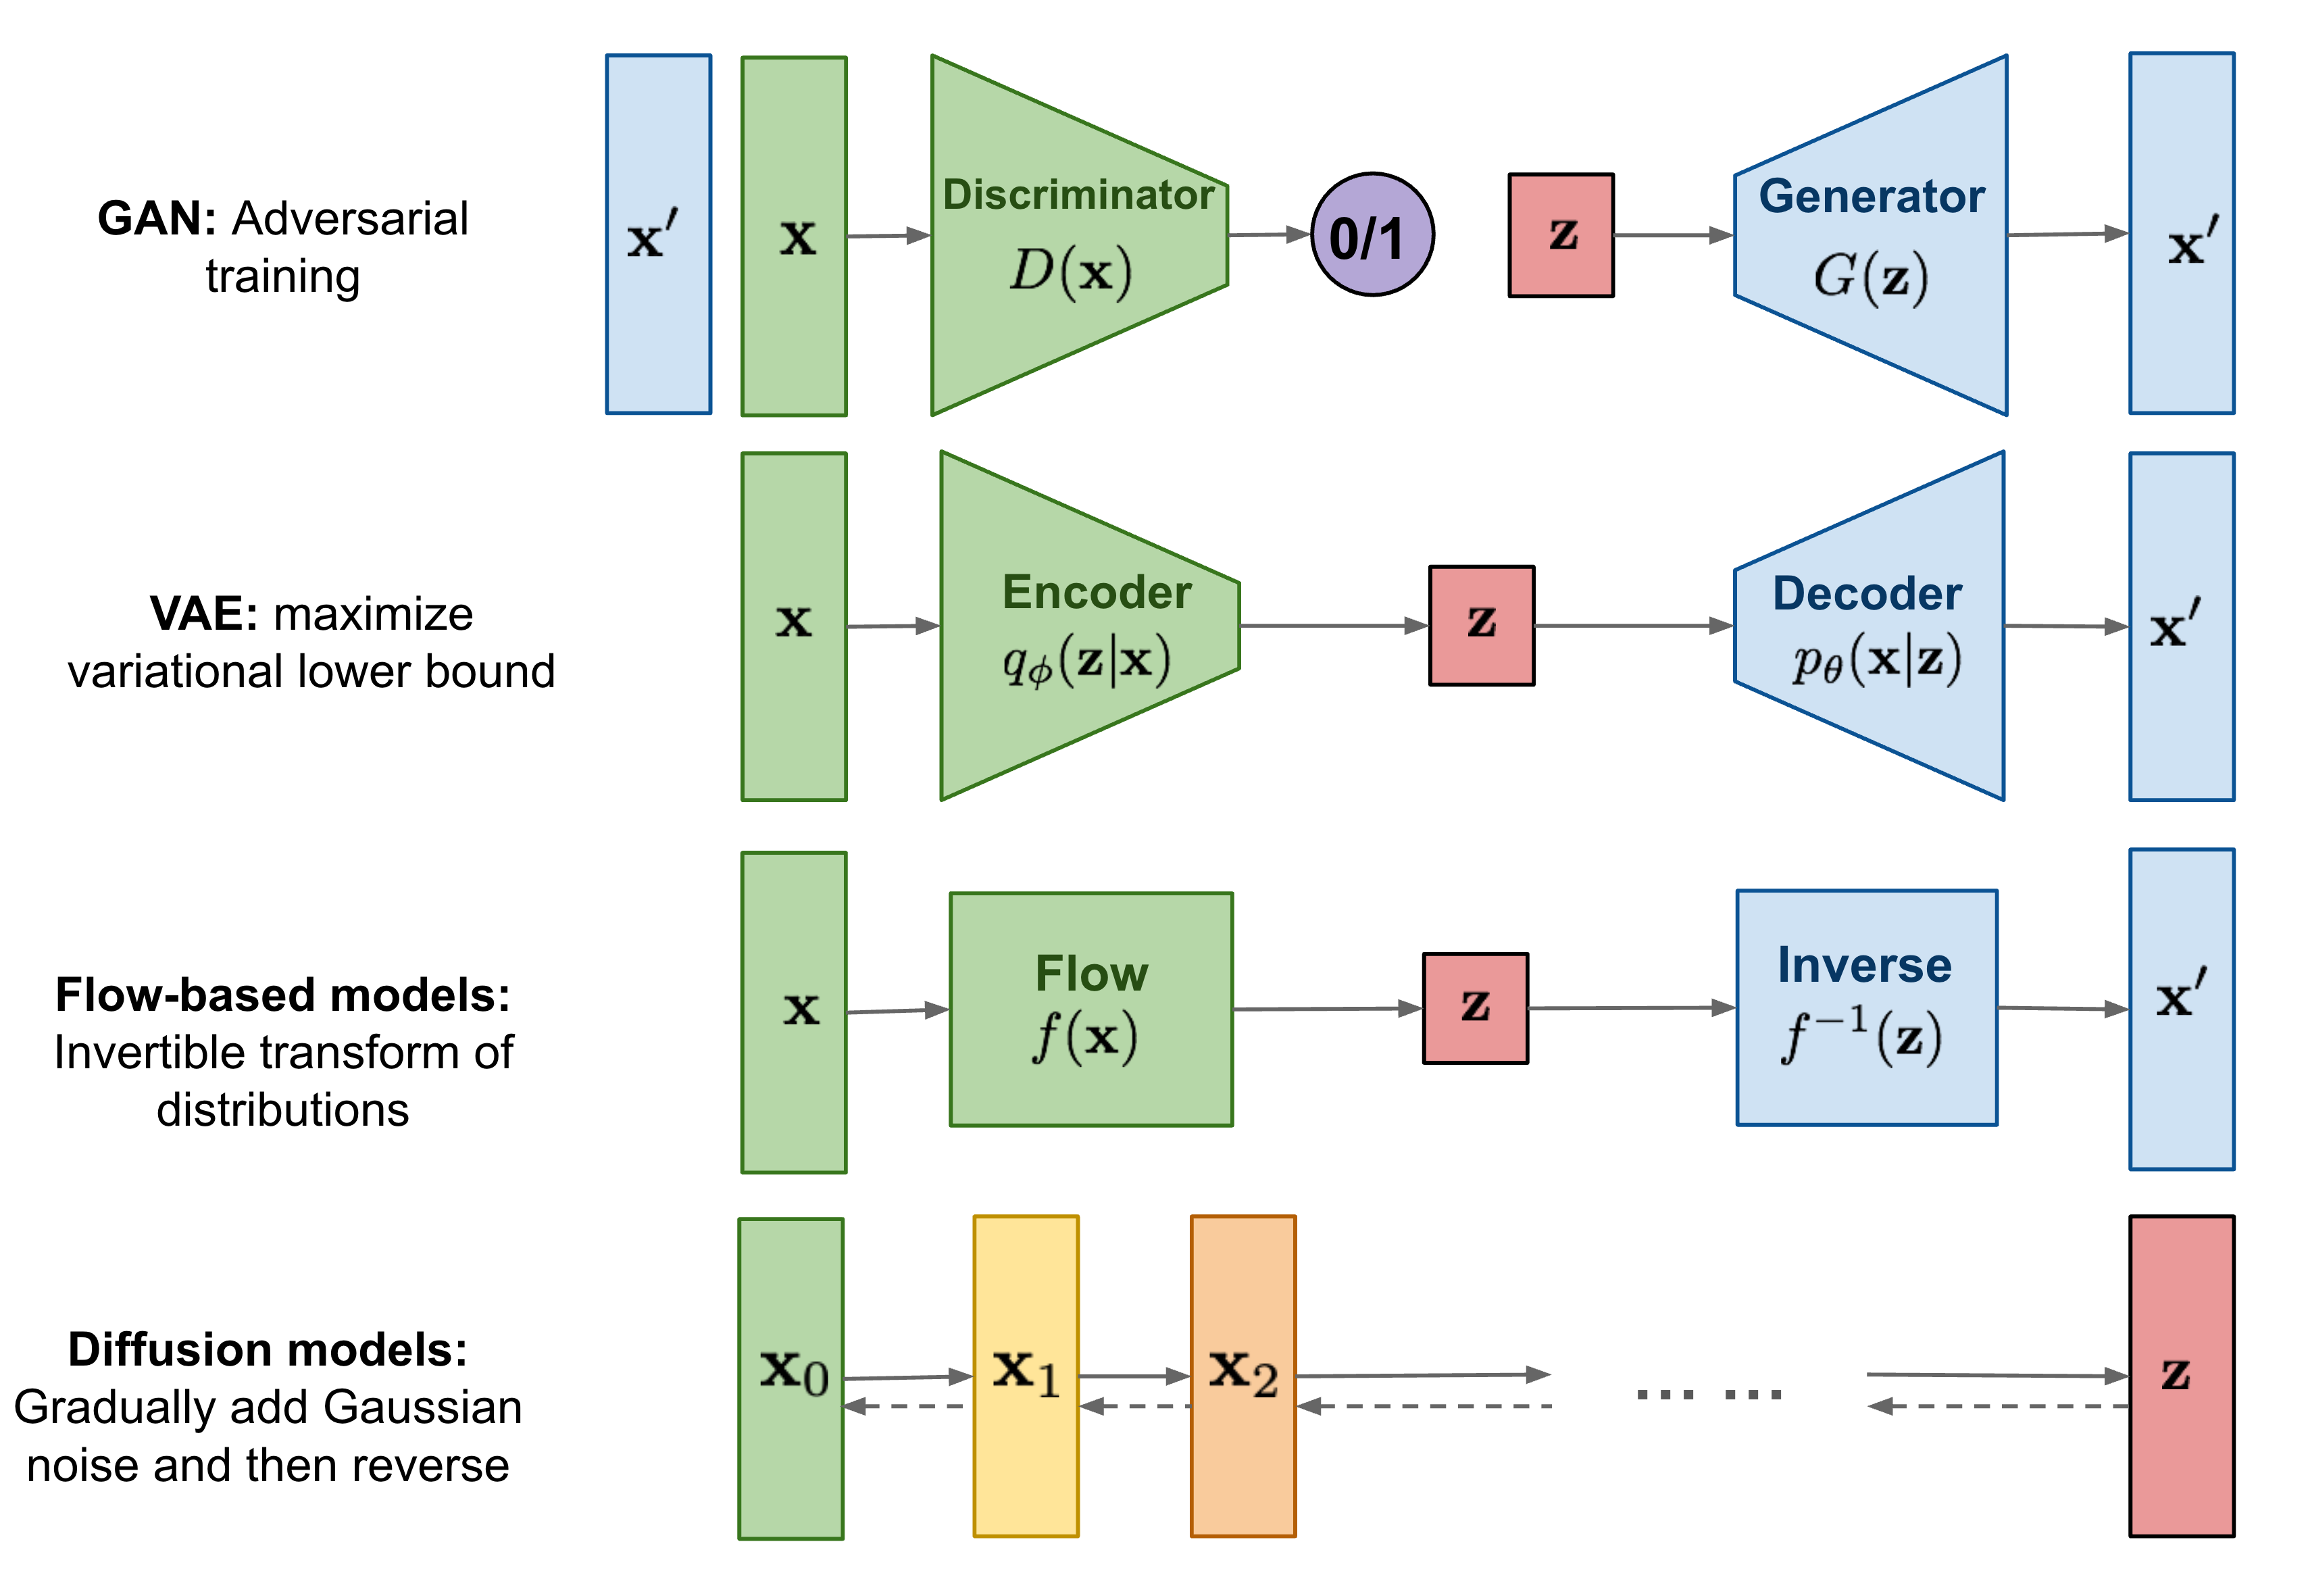
\includegraphics[width=\linewidth]{figs/generative-overview}
	\end{figure}
	\myfootnotewithlink{https://lilianweng.github.io/posts/2021-07-11-diffusion-models/}{Weng L. What are Diffusion Models?, blog post, 2021}
\end{frame}
%=======
\begin{frame}{The worst course overview :)}
	\begin{figure}
		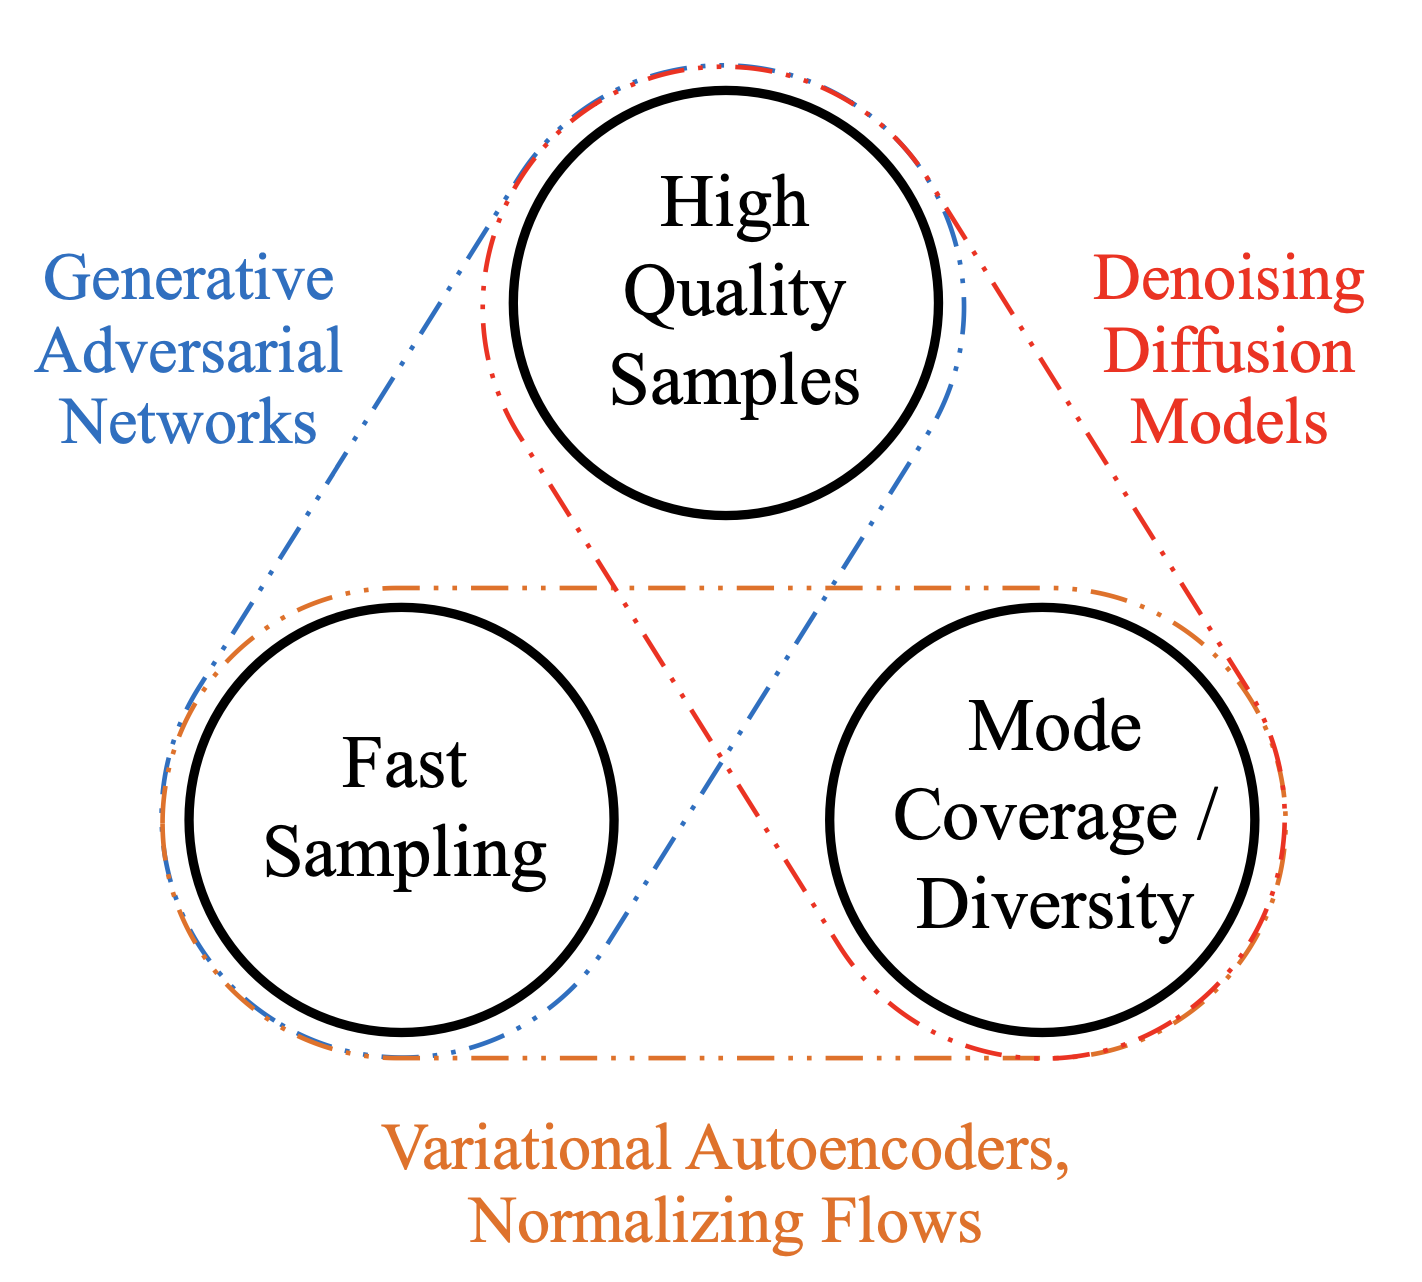
\includegraphics[width=0.7\linewidth]{figs/trilemma}
	\end{figure}
	\myfootnotewithlink{https://arxiv.org/abs/2112.07804}{Xiao Z., Kreis K., Vahdat A. Tackling the generative learning trilemma with denoising diffusion GANs, 2021}
\end{frame}
%=======
\begin{frame}{The worst course overview :)}
	\begin{figure}
		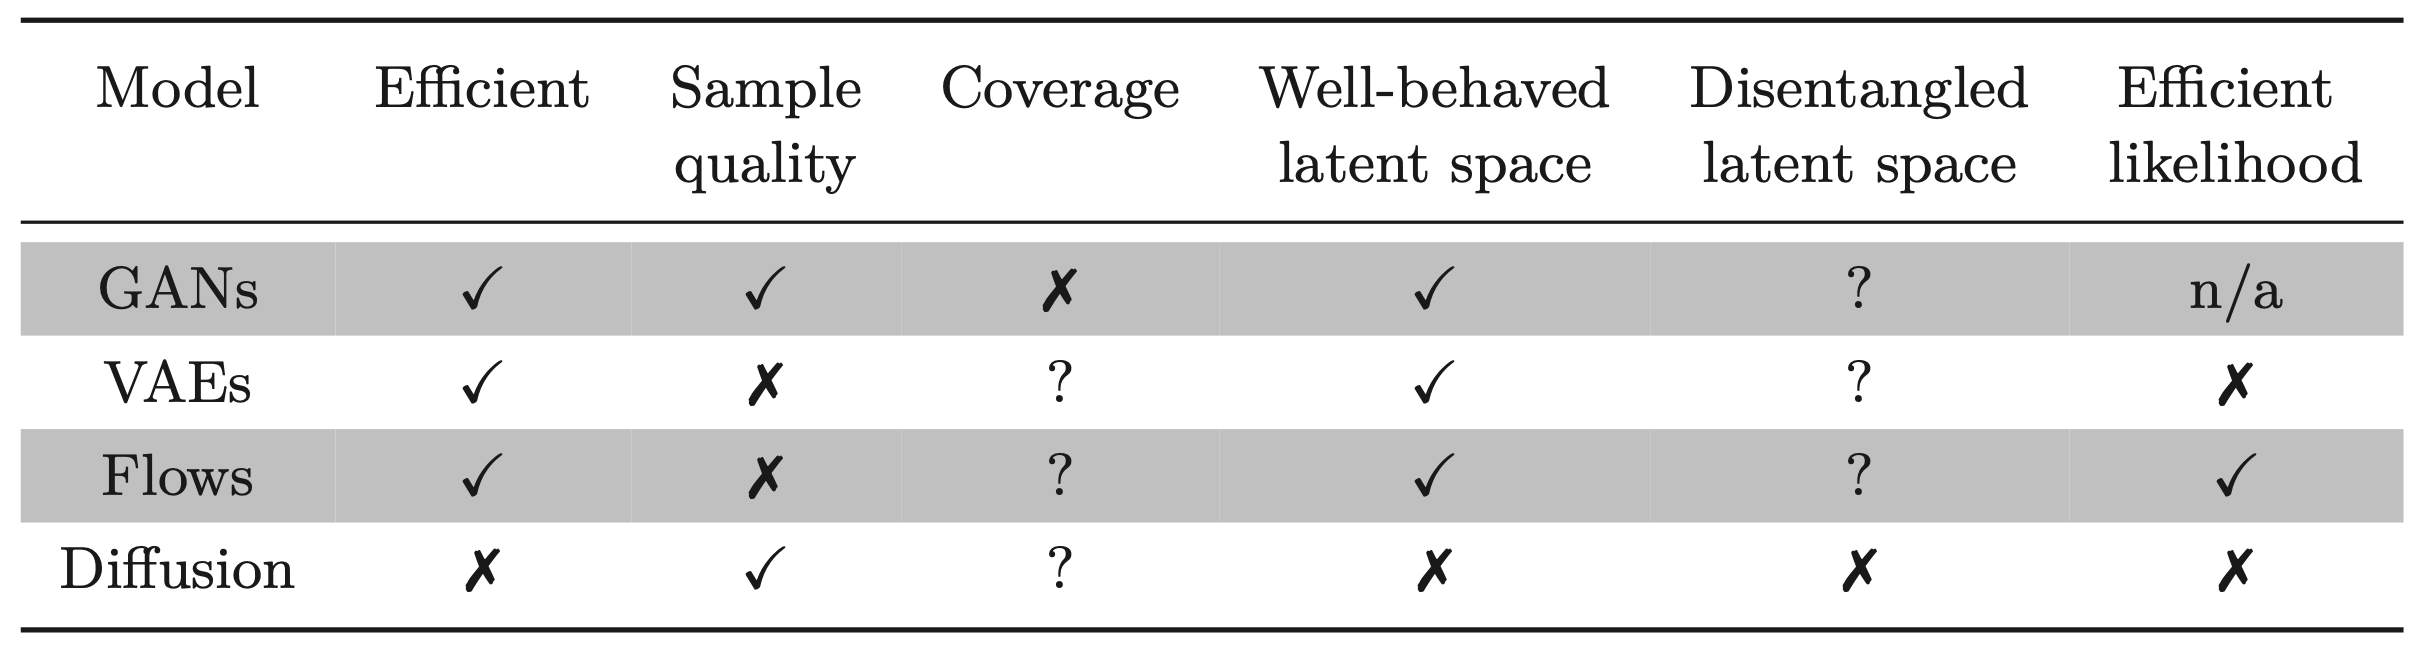
\includegraphics[width=\linewidth]{figs/gen_comp_table}
	\end{figure}
	\myfootnotewithlink{https://udlbook.github.io/udlbook/}{Simon J.D. Prince. Understanding Deep Learning, 2023}
\end{frame}
%=======
\begin{frame}{Summary}
	\begin{itemize}
		\item 
	\end{itemize}
\end{frame}
\end{document} 